\section{Architecture}
In this section dedicated to the architecture of the thesis, we will delve into the organizational framework of the foundational code derived from the GitHub repository \cite{LFighter_code}. We will discuss the structural elements that constitute the basis of our work, elucidating the positioning of the newly crafted code that serves the thesis purpose. The goal is to demonstrate how the intricate nature of a typical FL environment is mirrored in the architecture of this implementation by drawing comparisons to real-world FL scenarios and the base code structure.

%%%%%%%%%%%%%%%%%%%%%%%%%%%%%%%%%%%%%%%%%%%%%%%%%%%%%%%%%%%%%%%%%%%%%%%%%%%%%%%%%%%%%%%%%%%%%%%
\subsection{Base code structure} \label{sec:base_code}
The base code is implemented in Python and structured as follows:
\begin{itemize}
        \item Python notebooks (.ipynb files): There are three notebooks, one for each dataset used in the developer's experiments. The included datasets are:
        \begin{itemize}
                \item MNIST \cite{MNIST}: This dataset contains samples of handwritten digits. It consists of a training set of 60,000 samples, and a test set of 10,000 samples. Each sample is a 28x28 bit grayscale image, associated with a label from 10 classes. The task is to classify the images into their respective digit classes.
                \item CIFAR-10 \cite{CIFAR10}: This dataset contains 60,000 32x32 bit color images in 10 different classes. These classes encompass a diverse array of objects, including but not limited to animals, vehicles, and everyday items. The objective underlying this dataset is to accurately classify each image into its designated class.
                \item IMDB \cite{IMDB}: This dataset contains 50,000 movie reviews from the Internet Movie Database. The task is to classify the reviews into positive or negative sentiment.
        \end{itemize}
        The notebooks are used to run the experiments using the different aggregation functions commented in section \ref{sec:aggregation_methods} at user's will. This is done by importing the libraries and defining global variables in one executable section, and arranging the tests with different aggregation methods into separate sections. These notebooks are also used to visualize the results and checking the process.
        \item \textit{experiment\_federated.py}: This python file contains a sole function (\textit{run\_exp()}) that is called by one of the Python notebooks whenever we wish to start a new experiment with an aggregation function. This function merely prints by console information concerning the parameters used in the current experiment, initializes the FL environment and, calls a more complex function.
        \item \textit{environment\_federated.py}: This is the most complex file in the base code. It contains the \textit{run\_experiment()} function, which is the one called by the previous file. This function is responsible for the execution of the experiment, and it is where the whole FL setting is initialized and simulated. The file is divided into two main classes:
        \begin{itemize}
                \item Peer: When a Peer object is created, the Peer class initializes all its variables, such as the peer's ID, its local data, etc. This class contains a single function, named \textit{participant\_update()}, which is called when a peer has to update its local model. This function is responsible for the training of the local model, and it is where, depending on the value of the parameter "\textit{attack\_type}", the execution of the attack is determined. The function returns the updated local model.
                \item FL: This class is responsible for the initialization of the FL environment, from the most simple parameters such as the global rounds, to the more complex tasks such as creating the peers' instances and setting the global model up. It contains four functions:
                \begin{itemize}
                        \item \textit{test()}: This function is used to test the model's accuracy.
                        \item \textit{test\_label\_predictions()}: As the name suggests, this function is used to test the label predictions of the model received as a parameter. It is responsible for returning a list with the actual labels and another with the predicted ones in order to obtain the accuracy of the model.
                        \item \textit{choose\_peers()}: This function selects \textit{n} random peers from the list of peers. The value of \textit{n} is determined by the total amount of peers and the malicious rate, which is a floating-point variable.
                        \item \textit{run\_experiment()}: This is the function that simulates the whole FL environment. The function is built as follows:
                        \begin{enumerate}
                                \item It begins by copying the global model into a local variable.
                                \item After that, it iterates through a loop a total of "\textit{global\_rounds}" times. Inside this loop, for each global round, it selects the peers that will participate in the current round by calling the \textit{choose\_peers()} function, it also reinitializes the utility tables (weights, local models, etc.) of the peers that will participate in the current round, and then, for each peer participating:
                                \begin{enumerate}
                                        \item It defines the peer as attacker or regular depending on the output of \textit{choose\_peers()}, calls the \textit{participant\_update()} function of the peer.
                                        \item It updates the utility tables of the peer with the new values.
                                \end{enumerate}
                                \item After all peers have been updated, it aggregates the local models of the peers that participated in the current round by the selection of the aggregation function dependant on a series of conditional statements.
                                \item It updates the global model with the aggregated model and the process is repeated until the global rounds are completed.
                                \item The \textit{test()} function is called to obtain the model's accuracy.
                                \item Finally, it returns the system's state by console.
                        \end{enumerate}
                \end{itemize}
        \end{itemize}
\end{itemize}
The logical location for the newly created code, explained in Section \ref{sec:implementation} is inside the \textit{environment\_federated.py} file. The exact placement for these functions is inside the \textit{participant\_update()} function, contained by the Peer class.
This is because it is the single point of entry for the execution of the attack, and it is where the local model is updated.

%%%%%%%%%%%%%%%%%%%%%%%%%%%%%%%%%%%%%%%%%%%%%%%%%%%%%%%%%%%%%%%%%%%%%%%%%%%%%%%%%%%%%%%%%%%%%%%
\subsection{Real-world FL vs. base code}
In this section, we state the similarities between a real FL system and the base code described in the previous section, \ref{sec:base_code}. As a navigational aid as we navigate through the details of these two distinct environments, \autoref{fig:FL_diagram} provides a diagram of an actual FL scenario to further illuminate this comparison. 
\begin{figure}[h!]
        % \begin{figure}[H] % Alternative positioning
        \centering % sempre
        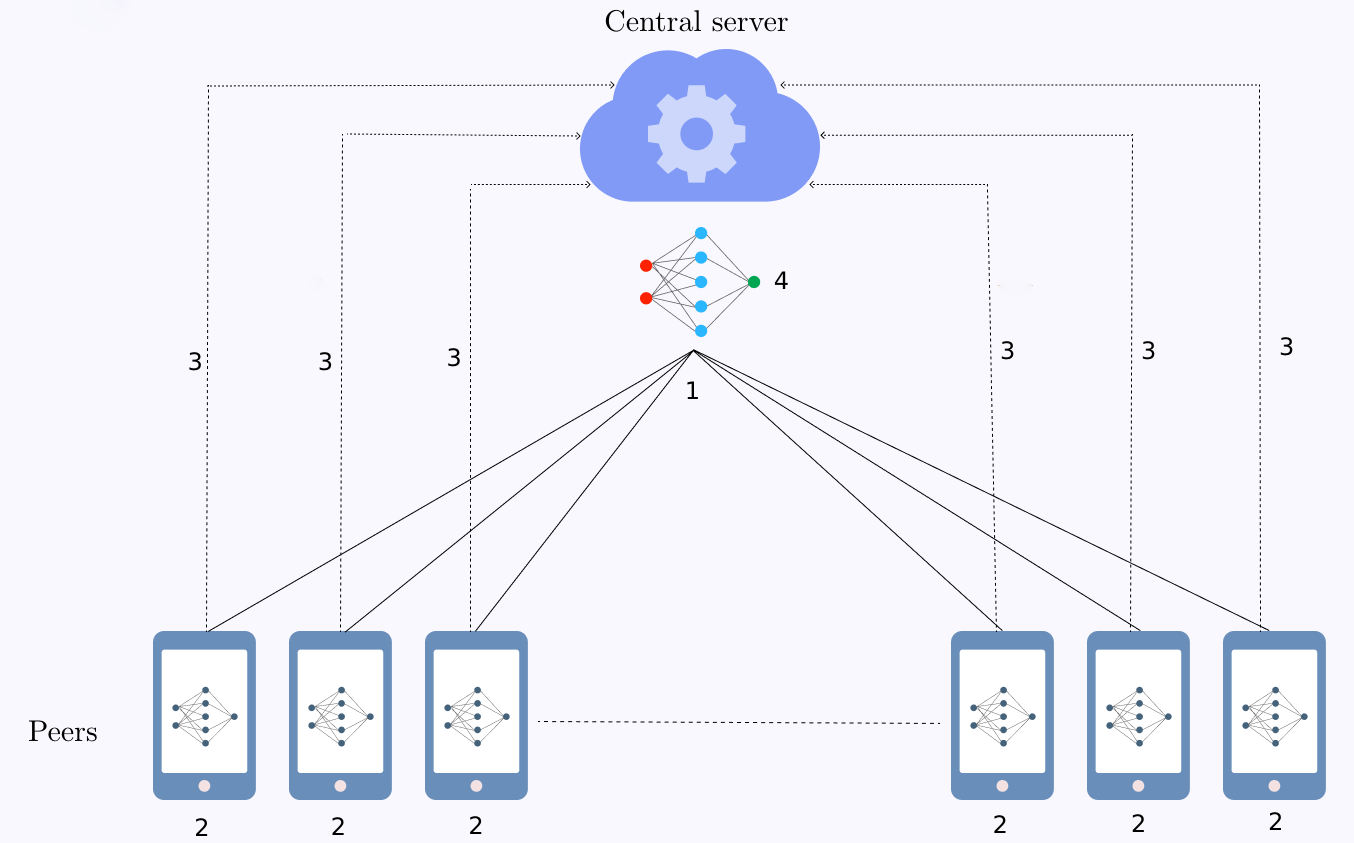
\includegraphics[scale=0.3]{FL_diagram.png}
        \caption{Federated Learning process. Source: \textit{Devfi}} % sempre
        \label{fig:FL_diagram}
\end{figure}

Next, the steps comprising the diagram are briefly outlined:
\begin{enumerate}
        \item The server sends the global model to the clients. This step is mirrored in the base code at the beginning of the \textit{run\_experiment()} function, which is responsible for the initialization of the FL environment, and it is where the global model is initialized and sent to the clients.
        \item The clients train the model with their local data. The second step exhibits its equivalence in the \textit{participant\_update()} function, which is called for each peer participating in the current round. This function is responsible for the training of the local model.
        \item The clients send the updated models to the server. This step is difficult to locate in the base code, as it is not explicitly stated. However, it is possible to infer that the updated models are sent to the server in the \textit{run\_experiment()} function, where the local models are located in table structures managed by the code.
        \item The server aggregates the models and sends the updated global model to the clients. This step is mirrored in the base code at the series of if statements mentioned in the previous section, \ref{sec:base_code}, which are responsible for the aggregation of the local models.
\end{enumerate}
The process is repeated until the global model converges. This step is mirrored in the loop defined in the \textit{run\_experiment()} function, which is dependant on the value of the parameter "\textit{global\_rounds}".


\pagebreak